\section{Attribute Editing in GAN Latent Spaces}

Modern Generative Adversarial Networks (GANs) have shown that the latent codes controlling image generation often embed rich semantic structure. 
In particular, many high-level attributes (e.g. age, smile, pose) correspond to almost-linear directions in the latent space \citep{shen2020interpretinglatentspacegans,härkönen2020ganspacediscoveringinterpretablegan}.
Once a direction vector $d$ for an attribute is found , editing is done by simple latent arithmetic $w_{edit} = w+\alpha d$
where $w$ is the original latent code $\alpha$ is a scalar step size, and $d$ is the learned attribute direction.
For example, InterFaceGAN treats attributes as binary labels and trains a linear SVM in the latent space; the normal vector of the separating hyperplane becomes $d$ \citep{shen2020interpretinglatentspacegans}. 
Style-based GANs (StyleGAN1/2) enhance this by using a mapping network to produce an intermediate latent 
$W$ space that is empirically more disentangled than the input 
$Z$ space \citep{karras2020analyzingimprovingimagequality,wu2020stylespaceanalysisdisentangledcontrols}.

There are two main approaches to finding attribute directions. 
Supervised methods use labeled data: for a given attribute one can train a linear classifier 
(e.g. on whether images have glasses) on a set of latent vectors. The classifier's weight vector 
(normal to the decision boundary) becomes the edit direction. InterFaceGAN demonstrated this works for many facial attributes \citep{shen2020interpretinglatentspacegans}.
There are two main approaches to finding attribute directions. Supervised methods use labeled data: for a given attribute one can train a linear classifier 
(e.g. on whether images have glasses) on a set of latent vectors. The classifier's weight vector (normal to the decision boundary) becomes the edit direction. InterFaceGAN demonstrated this works for many facial attributes.
Unsupervised methods do not require labels: GANSpace, for instance, collects many random latents and applies Principal Component Analysis to find dominant directions.
These principal axes often correspond to pose, lighting, or object type. Other factorization techniques, like SeFa, and style-space channel-searchers similarly find promising axes with little or no supervision \citep{shen2020interpretinglatentspacegans,härkönen2020ganspacediscoveringinterpretablegan,shen2021closedformfactorizationlatentsemantics}.

Once a direction $d$ is chosen,  editing is simply walking along that direction in latent space. Concretely, after inverting or sampling a code $w$, one produces an edited image by generating from
$w + \alpha d$ for various $\alpha$. 
InterFaceGAN likewise shows that adding the gender vector shifts a face's apparent gender. 
In general , Attribute Editing Models use the same principle of finding $d$ or $\Delta w$ and setting $w_{edit} = w + \alpha d$ to change
attributes in an image \citep{härkönen2020ganspacediscoveringinterpretablegan,shen2020interpretinglatentspacegans,li2023preim3d3dconsistentprecise,wu2020stylespaceanalysisdisentangledcontrols}

Importantly, these methods rely on latent disentanglement: the idea that different factors are (at least partly) separable. 
StyleGAN's design helps here: its intermediate latent $W$ is empirically more disentangled than the raw $Z$ space \citep{wu2020stylespaceanalysisdisentangledcontrols}.
StyleGAN2's per-channel style parameters (“StyleSpace”) have been shown to control very localized attributes (e.g. hair color, background elements) with minimal interference.
In contrast, earlier GANs had more entangled latents, making clean edits harder \citep{salehi2020generativeadversarialnetworksgans,Creswell_2018}.

However, disentanglement is not perfect. Most discovered directions still have residual cross-attribute effects. For example, 
one edit vector might change both “smile” and “age” together. This entanglement is noted in the literature: 
many control directions affect multiple attributes and can be “non-local” \citep{wu2020stylespaceanalysisdisentangledcontrols}.
To mitigate this, some methods perform conditional manipulation: e.g. subtracting out the projection of one direction on another to isolate each effect. 
But instability remains when editing multiple attributes at once, often producing unrealistic images if not handled carefully.

Attribute editing assumes that one has latent code $w$ to edit . To apply editing to real photos, a critical step is GAN inversions. 
By finding a latent code that faithfully reproduces a given real image, one can apply learned semantic manipulations 
,adjusting age, hairstyle, or pose, to that image \citep{bobkov2024devildetailsstylefeatureeditordetailrich,alaluf2021restyleresidualbasedstyleganencoder}.
We find a latent code $z^*$ whose generator output matches the target image. Once $z^*$ is found , one can apply
the $w_{edit}$ formula to manipulate the image attributes.
According to \citet{xia2022ganinversionsurvey}, there 2 gan inversion methods. Namely, the learning-based(encoder-based) and optimization based Gan inversions.
\begin{itemize}
    \item Optimization-based inversion solves for $z^*$ by backpropagation: it iteratively adjusts $z$ to minimize reconstruction loss $||G(z)-x||$ This often yields high-fidelity reconstructions but can be slow and may get stuck in local minima.
    \item Learning(Encoder)-based trains a neural network $E(\cdot)$ to map images to latent codes. A trained encoder can invert images quickly, though it must be carefully regularized to align with the pretrained generator. Hybrid approaches use an encoder for an initial guess followed by optimization refinement \citep{xia2022ganinversionsurvey}.
\end{itemize}

GAN inversion is what allows editing of real images. For instance, the survey by \citet{xia2022ganinversionsurvey} 
illustrates how an inverted code $z^*$ can be altered by adding attribute vectors  $n_1,n_2$ to change the age or smile of a real face.
They note that after inversion, the same latent-space editing techniques apply “without requiring any ad-hoc supervision”
However , inversion quality has limits: early models like Progressively Growing Gan (PGGAN)\citep{karras2018progressivegrowinggansimproved} were hard to invert faithfully,
whereas StyleGAN's architecture yields much better inversions \citep{karras2020analyzingimprovingimagequality}. 
Imperfect inversion can blur details or introduce artifacts, which in turn limits how well edits carry over to the final image.

\subsection{Attribute Group Editing}

Beyond single images, recent work uses latent editing for few-shot image generation: synthesizing new images of a novel category given only a few examples. The idea is to treat each new class as a 'set of attributes' and apply the learned edit directions to produce more samples. A pioneering approach is Attribute Group Editing (AGE) \citep{AGE}.
AGE assumes that images are combinations of category-relevant and category-irrelevant attributes. It represents a category by its class embedding $w_c$: the mean latent of the few examples.
The attributes that define the category (e.g., animal shape) are captured in $w_c$. 
AGE then learns a sparse dictionary of category-irrelevant attribute directions (e.g. fur color, pose) by doing sparse coding on the differences
$w_{sample}-w_c$ for many samples.  The key assumption is that an attribute direction (such as 'smiling' or 'red flower') is shared between categories.
To generate new images of an unseen category, AGE starts with the class embedding $w_c$
and adds combinations of these dictionary directions, creating diverse variations while keeping the features of the core category fixed.
This editing-based generation requires no GAN retraining and can produce high-quality, diverse images even from one or few inputs.

\begin{figure}[htbp]
    \centering
    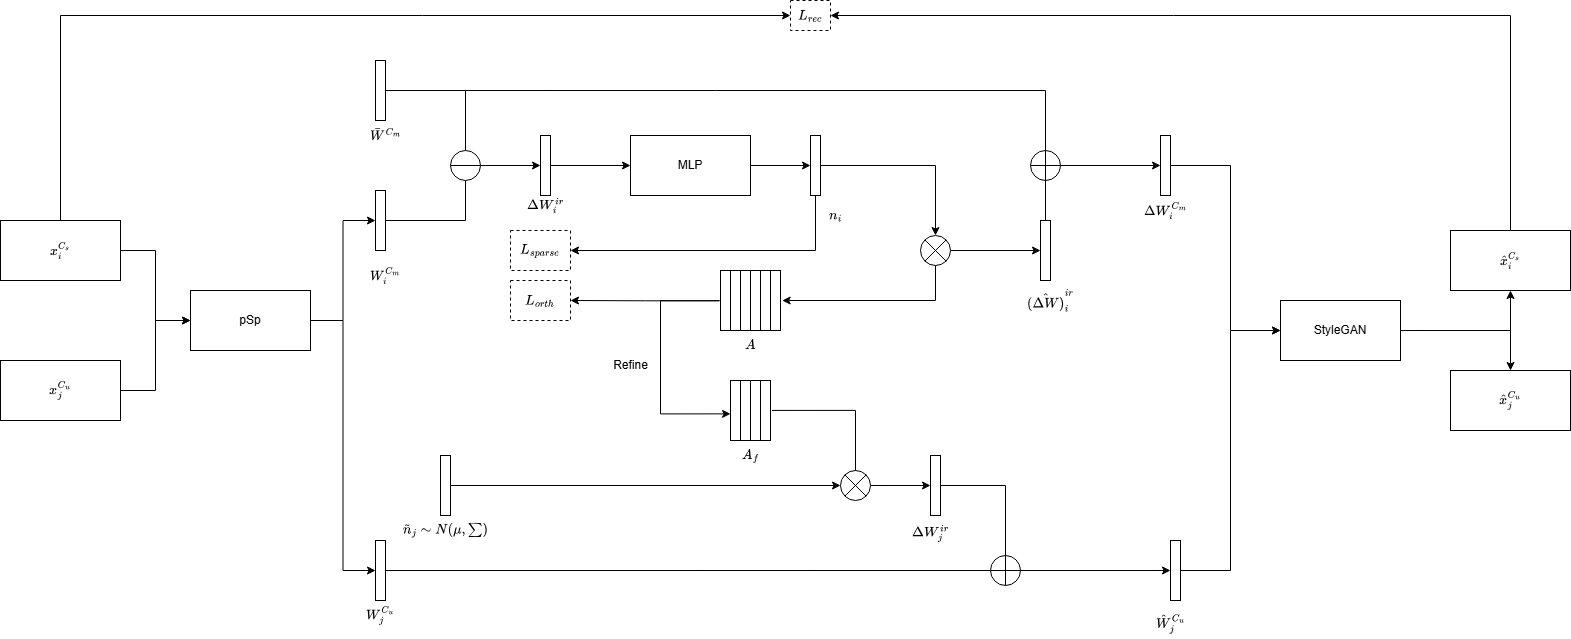
\includegraphics[width=1\linewidth]{figures/age_framework.png}
    \caption{\textit{Attribute Group Editing Framework}}
    \label{fig:AGEframework}
\end{figure}

AGE provides a powerful framework, but has some limitations. The SAGE (Stable AGE) follow-up
aims to improve class consistency. Instead of editing from just one example, SAGE uses all a few-shot images to robustly estimate the class embedding. 
It leverages the same attribute dictionaries but selects appropriate directions based on the new class's similarity to the seen classes.
In effect, SAGE 'injects the whole distribution of the novel class into StyleGAN's latent space', preserving the identity of the category.
This leads to more stable outputs that help downstream tasks (e.g., classification) perform better on the generated images \citep{ding2023stableattributegroupediting}.

Most recently, TAGE (Trustworthy AGE) has extended this line further. TAGE also uses a codebook (dictionary) of attributes, but introduces transformer-style modules. Its Codebook Learning Module (CLM) finds semantic directions for category-related and unrelated attributes and builds a sparse dictionary.
A Code Prediction Module (CPM) then uses global combinatorial reasoning (long-range attention) to predict the best edit codes for a given few-shot class, improving diversity and accuracy. Crucially, TAGE adds a Prompt-Driven Semantic Module (PSM): it generates textual or semantic prompts that are injected into transformer layers, guiding fine-grained editing \citep{zhang2024tagetrustworthyattributegroup}.

\subsection{Stable Attribute Group Editing}

Stable Attribute Group Editing (SAGE) was proposed as a method to overcome such limitations of AGE. Instead of editing from a single exemplar, SAGE initially employs all the given few-shot images to estimate a stable class-center embedding. It does so by capitalizing on the pretrained category-relevant attribute dictionary (learned from visible classes) to linearly represent the novel class centroid in the latent space. As described by Ding et al., since there are not a sufficient number of examples to calculate a credible mean directly, "the category-relevant dictionary… is complete enough to cover the unique attributes of any related categories," a linear combination of the dictionary atoms can "recover the class-specific features of the unseen classes" \citep{ding2023stableattributegroupediting}.

In practice, SAGE projects the few-shot samples onto such an attribute dictionary to separate their shared class features from each other, essentially removing the attributes not related to categories and retaining the attributes that are related. According to the authors, such a disentanglement also helps the model to estimate a more accurate class embedding even for a very small number of samples. The experiments also indicate that the estimated embedding from only three face images well approximates the ground truth centroid over hundreds of actual instances.

In the same paper, the weights from the projection are utilized for adaptively choosing which category-irrelevant editing directions to use. Taking cues from biological taxonomy, the authors make the assumption that categories sharing the same relevant characteristics which is being members of the same genus, for example they also share compatible and safe irrelevant characteristics. Consequently, SAGE picks the category-irrelevant directions from the highly similar seen classes depending on the projection coefficients. The approach enables the method to introduce the distribution of the unseen class to StyleGAN’s latent space by essentially repositioning the generated sample cloud towards the actual class manifold. Anchoring the synthesis about this reconstructed embedding and then carrying out filtered edits, SAGE manages to maintain class identity despite generating diverse and realistic variations.

This refinement of AGE yields clearer gains in category consistency and diversity. Quantitative results show that SAGE produces samples with significantly better quality (lower FID) and greater diversity (higher LPIPS) than AGE and competing few-shot methods. For example, without retraining the GAN, “SAGE generates images with higher quality and diversity” than prior fusion- or transformation-based approaches, and its class-embedding mapping makes it “much more stable than AGE”. Qualitatively, Ding et al. illustrate that AGE could produce bizarre artifacts (a “cat with a dog nose” or a “bird with two heads”) when editing from extreme inputs, whereas SAGE’s tailored embedding and adaptive edits yield realistic variants without such errors. In the latent space of an unseen class, AGE’s few-shot samples often lie at extreme positions and its generated points cluster narrowly around them. By contrast, SAGE’s injections form a much wider latent cloud that more closely matches the true distribution. The authors summarize that SAGE “relocates the whole distribution of the novel class in the latent space, thus effectively avoiding category-specific editing and enhancing the stability”. In downstream classification tasks, this translates into higher Naive Augmentation Scores than AGE: across several datasets SAGE’s synthetic data boosts accuracy over AGE and fusion-based methods. For example, on a bird dataset SAGE improves NAS from 42\% (AGE) to 46\%, even approaching the fully supervised baseline of 52\%. Overall, Ding et al. report that SAGE achieves “more stable and reliable few-shot image generation” with significantly better category retention than previous methods.

Nonetheless, SAGE does not solve all challenges. The authors note that its generative range is still more restricted than that of real data: the “dynamic range” of editable variations in SAGE is smaller than in the true class. In practice, SAGE currently uses a uniform editing intensity for all directions (since estimating per-attribute scales from few samples is infeasible) and its dictionary contains only attributes that recur across the seen classes. Consequently, some subtle class-specific variations may still be missing. As the paper observes, “SAGE simply assumes a unified intensity for editing direction sampling,” and capturing attribute-dependent editing amplitudes or class-specific edits remains an open issue. Moreover, while classification performance is improved over AGE, it still generally lags behind a model trained on real examples. This gap – and the reliance on a pretrained StyleGAN inversion as the generator – highlight future work: extending SAGE’s ideas to handle multi-scale attributes and other generative models may be needed to fully close the gap for few-shot tasks.

\subsection{Datasets and Applications}

Attribute editing techniques are typically developed and evaluated on diverse image domains. 
Face datasets (CelebA, FFHQ, VGGFace) are common: they have many labeled attributes and StyleGAN 
models are readily available for them. 
Few-shot generation research has also expanded to other domains. 
For instance, the Flowers dataset has 102 flower species \citep{gupta2024conditionaldistributionmodellingfewshot},
Animal Faces (or AnimalFacesHQ) has 149 animal species, VGGFace contains ~2300 human identities , and NABirds covers 555 North American bird species. 
These datasets test how well latent editing generalizes beyond human faces. 

Latent editing has practical use in data augmentation (few-shot generation) 
and interactive image manipulation. For example, 
one can start with a single bird photo and synthesize 
variants by editing color, pose, or environment using learned directions. 
StyleGAN models have even been trained on NABirds to allow such editing of 
feathers or backgrounds (though this is still an active research area). 
However, note that many attributes in faces (smile, glasses, gender) 
do not directly map to birds or flowers; cross-domain transfer of semantic concepts remains challenging.



\subsection{Attribute Editing limitations and challeges}

Despite their promise, latent-space attribute editing methods face several challenges \citep{wu2020stylespaceanalysisdisentangledcontrols,AGE,ding2023stableattributegroupediting,shen2020interpretinglatentspacegans,xia2022ganinversionsurvey,liu2023delvingstyleganinversionimage}:

\begin{itemize}
    \item Attribute entanglement. Discovered directions often change multiple features at once. For instance, moving along an “age” vector might also alter “expression”. Entangled edits require careful design (e.g. subtracting projections) or more sophisticated disentanglement techniques. Fully disentangling a GAN’s latent space is still an open problem.
    \item Multi-attribute interactions. Applying more than one edit vector can be unstable. Sequential edits may accumulate artifacts, and combining directions (e.g. “add glasses” and “increase smile”) can produce unrealistic results if the attributes interact in complex ways. Ensuring consistent multi-attribute editing (for example, editing several facial features simultaneously without distortion) remains tricky.
    \item Inversion quality. Editing real images relies on GAN inversion. If the inversion does not perfectly capture the original, edits may fail or degrade fidelity. Early GANs (like PGGAN) struggled with inversion.While StyleGAN produces better inverted results, truly lossless inversion is hard. Any residual reconstruction error limits how cleanly attributes can be edited.
    \item Generalization to diverse datasets. Most latent-editing research has centered on well-studied domains (faces, common objects). Extending these methods to fine-grained categories like birds or flowers raises issues. The learned GAN (or its latent semantics) may not capture useful directions in these domains, especially if attribute labels are scarce. Additionally, attributes meaningful in one domain (e.g. “nose shape” in faces) do not translate to others. New methods must learn or adapt directions that make sense for non-face classes.
\end{itemize}